\documentclass{article}
% Essential packages
\usepackage{graphicx}
\usepackage{comment}
\usepackage{amssymb}
\usepackage{amsmath}
\usepackage{amsthm}
\usepackage{graphicx}
\usepackage{float}
\usepackage{comment}
\usepackage{caption}
\usepackage{multirow}
\usepackage{listings}
\usepackage{xcolor}
\usepackage[hidelinks]{hyperref}
\usepackage{enumitem}
\usepackage{titlesec}
\usepackage{algorithm}
\usepackage{algpseudocode}
\usepackage{tcolorbox} 
\usepackage{fancyhdr}
\usepackage{mdframed} 
\usepackage{tikz}
\usetikzlibrary{arrows.meta, calc, positioning, backgrounds, shapes.geometric, fit}
\usepackage{pgfplots}

% Command to get the current month name
\newcommand{\MonthName}{
  \ifcase\month\or January\or February\or March\or April\or May\or June\or July\or August\or September\or October\or November\or December\fi}
  
% Configurazione di codeblocks con il pacchetto listings
\lstset{
  basicstyle=\ttfamily\small,
  keywordstyle=\color{blue},
  commentstyle=\color{green!50!black},
  stringstyle=\color{red},
  showstringspaces=false,
  breaklines=true,
  frame=single, % Adds a border around the code
  numbers=left, % Line numbers on the left
  numberstyle=\tiny\color{gray}, % Style of line numbers
  stepnumber=1, % Number of lines to skip between numbers
  numbersep=-5pt, % Distance between line numbers and code
  tabsize=2, % Tab size
  captionpos=b, % Position of the caption
}

% Header configuration
\pagestyle{fancy}
\fancyhf{} % Clean header and footer
\fancyhead[L]{\leftmark} % Current section on the top left
\fancyhead[R]{\thepage} % Page number on the right

% Defines a command for framed definitions with a blue background and a title
\newcommand{\definition}[2]{%
\begin{mdframed}[
    hidealllines=false,
    linecolor=blue!80!black,
    linewidth=1pt,
    backgroundcolor=blue!5,
    roundcorner=5pt,
    frametitle={#1},
    frametitlebackgroundcolor=blue!80!black,
    frametitlefont=\color{white}\bfseries,
    innerbottommargin=10pt,
    skipabove=10pt,
    skipbelow=10pt
  ]
  {#2}
  \end{mdframed}
}

% Defines a command for framed Note boxes with green background and a title
\newcommand{\note}[1]{%
\begin{mdframed}[
    hidealllines=false,
    linecolor=green!80!black,
    linewidth=1pt,
    backgroundcolor=green!5,
    roundcorner=5pt,
    frametitle={Note},
    frametitlebackgroundcolor=green!80!black,
    frametitlefont=\color{white}\bfseries,
    innerbottommargin=10pt,
    skipabove=10pt,
    skipbelow=10pt
  ]
  {#1}
  \end{mdframed}
}

% Make proof keyword bold
\makeatletter
\def\proofname{\bfseries Proof}
\makeatother
% PGFPlots settings
\pgfplotsset{compat=1.18}

%tikz styles for Bayesian Networks graphs
\tikzset{
  bn-node/.style={circle, draw=red, thick, minimum size=14pt},
  bn-arrow/.style={->, red, thick},
  bn-theta/.style={circle, draw=red, thick, minimum size=14pt, fill=blue!60},
  % D-separation styles
  dse-node-empty/.style={circle, draw=red, fill=orange!10, minimum size=6mm, inner sep=0pt},
  dse-node-filled/.style={circle, draw=red, fill=blue!60, minimum size=6mm, inner sep=0pt},
  dse-indep-bg/.style={ellipse, fill=yellow!25, draw=black, thick, minimum width=7.5cm, minimum height=2.8cm},
  dse-dep-bg/.style={ellipse, fill=green!30, draw=black, thick, minimum width=7.5cm, minimum height=2.8cm},
  dse-small-indep/.style={ellipse, fill=yellow!25, draw=black, thick, minimum width=2.8cm, minimum height=2.2cm},
  dse-small-dep/.style={ellipse, fill=green!30, draw=black, thick, minimum width=2.8cm, minimum height=2.2cm},
  dse-boundary/.style={ellipse, draw=black, dashed, minimum width=3cm, minimum height=6.5cm},
  %Perceptron
  input-node/.style={rectangle, draw, minimum size=0.8cm},
  sum-node/.style={draw, fill=yellow!20, minimum size=1cm, thick},
  activation-node/.style={draw, fill=green!10, minimum size=1cm, thick},
  connection/.style={->, >=stealth, thick},
  dot/.style={circle, fill, inner sep=1.5pt},
  %SVM
  svm-blue_sq/.style={rectangle, fill=blue!80, inner sep=2.5pt},
  svm-red_circ/.style={circle, fill=red!80, inner sep=2.5pt},
  svm-blue-hidden_sq/.style={rectangle, fill=blue!80, inner sep=2.5pt, opacity=0.25},
  svm-red-hidden_circ/.style={circle, fill=red!80, inner sep=2.5pt, opacity=0.25}
}
\numberwithin{equation}{section} % Equations are numbered per section

\title{\Huge \textbf{Machine Learning}\\ \Large{Passerini Andrea\\a.y. 2025/2026\\University of Trento\\[2cm]}}
\author{Davide Donà}
\date{
    \MonthName\ \number\year \\[0.5em]
    \small\textcolor{gray}{\href{https://github.com/446f6e6e79/Machine-Learning-Notes}{Notes Repository}}
}
\begin{document}
% Set the page numbering to roman numerals
\pagenumbering{roman}

% Title and table of contents
\maketitle
\newpage
\tableofcontents
\newpage

% Change the page numbering to arabic
\pagenumbering{arabic}
\include{sections/Introduction}
\include{sections/DecisionTree}
\include{sections/K-Nearest-Neighbours}
\include{sections/Evaluation}
\include{sections/ParameterEstimation}
\include{sections/BayesianNetwork}
\include{sections/LearningBN}
\section{Naive Bayes}
Naive Bayes is a simple classification algorithm based on Bayesian networks.
\paragraph{Setting}
\begin{itemize}
    \item Each instance $x$ is represented by a set of attributes values $\langle a_1, a_2, \ldots, a_m \rangle$;
    \item The target feature $y$ is the class label we want to predict. It can take any value from a finite set $\mathcal{Y}$;
    \item The task is predicting the Maximum A Posteriori (MAP) estimate for the class label $y$ given the attribute values.
    In other words, we want to predict the class $\hat{y}$ that maximizes the posterior probability $P(y | a_1, a_2, \ldots, a_m)$.
    More formally:
    \begin{equation}
        \hat{y} = \arg\max_{y_i \in \mathcal{Y}} P(y_i | a_1, a_2, \ldots, a_m)
    \end{equation}
    Using Bayes' theorem, we can rewrite this as:
    \begin{equation}
        \hat{y} = \arg\max_{y_i \in \mathcal{Y}} \frac{P(a_1, a_2, \ldots, a_m | y_i) P(y_i)}{P(a_1, a_2, \ldots, a_m)}
    \end{equation}
    Since the denominator is constant with respect to $y_i$, we can simplify this to:
    \begin{equation}
        \hat{y} = \arg\max_{y_i \in \mathcal{Y}} P(a_1, a_2, \ldots, a_m | y_i) P(y_i)
    \end{equation}
\end{itemize}

\subsection{Naive Bayes assumption}
As the number of attributes increases, estimating the joint probability $P(a_1, a_2, \ldots, a_m | y_i)$ becomes increasingly difficult.
To simplify this, Naive Bayes makes the assumption that all attributes are independent of each other, given the class label $y_i$.
We can simplify the MAP estimate to:
\begin{equation}
    p(a_1, \ldots, a_m | y_i) = \prod_{j=1}^{m} P(a_j | y_i)
\end{equation}
This heavily reduces the number of parameters we need to estimate, making the model more efficient and less prone to overfitting.

\subsection{Naive Bayes classifier}
Given the assumption of conditional independence, the MAP estimate for the class label becomes:
\begin{equation}
    \hat{y} = \arg\max_{y_i \in \mathcal{Y}} \prod_{j=1}^{m} P(a_j | y_i) P(y_i)
\end{equation}
We assume that each value of attribute $A_j$ is modeled using the same type of distribution.
The probability of an attribute value given the class label $P(a_j | y_i)$ can for example be modeled 
using a multinomial distribution over the $k$ possible values of attribute $A_j$:
\begin{equation}
    P(a_j | y_i) = \prod_{k = 1}^{K} \theta_{kyi}^{z_k(a_j)}
\end{equation}
Where:
\begin{itemize}
    \item $\theta_{ky_i}$ is the parameter representing the probability of attribute $a_j$ taking value $k$, given class label $y_i$;
    \item $z_k(a_j)$ is an indicator function that is 1 if attribute $a_j$ takes value $k$, and 0 otherwise.
\end{itemize}

\subsubsection{Parameter estimation}
We need to estimate both the class prior probabilities $P(y_i)$ and the conditional probabilities $P(a_j | y_i)$ from the training data.
\begin{itemize}
    \item The class prior probabilities $p(y_i)$ can be easily learned as the fraction of training instances having each class label;
    \item The maximum likelihood estimate for the parameters $\theta_{ky_i}$ can be computed as the relative 
    frequency of attribute $A_j$ taking value $k$ among all instances with class label $y_i$.
    More formally:
    \begin{equation}
        \theta_{ky_i}^{\max} = \frac{N_{ky_i}}{N_{y_i}}
    \end{equation}
\end{itemize}
As previously mentioned, we can also introduce Dirichlet priors over the parameters to avoid zero probabilities for unseen attribute values:
\begin{equation}
    \theta_{ky_i}^{\max} = \frac{N_{ky_i} + \alpha_{ky_i}}{N_{y_i} + \alpha_{c}}
\end{equation}

\subsection{Example - Text Classification}
We want to classify documents into one of $C$ possible classes, based only the words they contain.
Let $V$ be the vocabulary of all possible words and $D$ a dataset of labeled documents.
\begin{itemize}
    \item We can easily compute the prior probabilities for each class $y_i$ as:
    \[
        P(y_i) = \frac{|D_i|}{|D|}
    \]
    \item We can model attributes with a multinomial distribution over $K = |V|$ possible words.
    \item The parameters $\theta_{ky_i}$ can be estimated as:
    \[
        \theta_{ky_i}^{\max} = \frac{\sum_{x\in D_i} \sum_{j = 1}^{|x|} z_k(x_j)}{\sum_{x \in D_i} N_{y_i}(x)}
    \]
    Where:
    \begin{itemize}
        \item $x$ is a document in the dataset;
        \item $D_i$ is the subset of documents in class $y_i$;
        \item $x_j$ is the $j$-th word in document $x$;
        \item $\sum_{x\in D_i} \sum_{j = 1}^{|x|} z_k(x_j)$ is the total number of occurrences of word $k$ in all documents of class $y_i$;
        \item $\sum_{x \in D_i} N_{y_i}(x)$ is the total number of words in all documents of class $y_i$.
    \end{itemize}
\end{itemize}
We can then classify a new document by computing the posterior probability for each class and selecting the class with the highest probability.
\begin{equation}*
    \hat{y} = \arg\max_{y_i \in \mathcal{Y}} \prod_{j=1}^{|x|} P(x_j | y_i) P(y_i) 
\end{equation}
Substituting the multinomial model for $P(x_j | y_i)$ and the prior $P(y_i)$, we get:
\begin{equation}
    \hat{y} = \arg\max_{y_i \in \mathcal{Y}} \prod_{j=1}^{|x|} \prod_{k = 1}^{K} \theta_{ky_i}^{z_k(x_j)} \cdot \frac{|D_i|}{|D|}
\end{equation}
\include{sections/LinearDiscriminantFunctions}
\include{sections/Perceptron}
\include{sections/SVM.tex}
\section{Kernel Machines}
With what we have seen so far about SVMs, we find out that:
\begin{itemize}
    \item \textbf{Hard Margin SVMs} can address linearly separable data only, with no misclassification;
    \item \textbf{Soft Margin SVMs} can address linearly separable problems with some degree of misclassification;
    \item \textbf{Non-linearly separable problems} need higher expressive power to be addressed.
\end{itemize}
\textbf{Kernel Machines} are an extension of SVMs that can address non-linearly separable problems, 
maintaining the same underlying principles of SVMs (large margin and theoretical guarantees).
\\The key idea is to \textit{map} the input data into a higher dimensional feature space, where it is more likely 
to be linearly separable and perform a linear separation in that space.
\subsection{Feature Map}
\definition{Feature Map}{
    \[
        \phi: \mathcal{X} \rightarrow \mathcal{H}
    \]
    A feature map $\phi$ is a function that maps the input space $\mathcal{X}$ to a higher dimensional 
    (possibly infinite-dimensional) feature space $\mathcal{H}$.
    \\\\All the examples $\boldsymbol{x}_i$ are replaced by their images $\phi(\boldsymbol{x}_i)$ in the feature space. 
    This should increase the expressive power of the representation, introducing features that are 
    combinations of the original inputs. In this new space, the data may become linearly separable.
}
An example of feature map is the following:
\definition{Polynomial Feature Map}{
    \begin{itemize}
        \item \textbf{Homogeneous Polynomial Feature Map} of degree $2$:
    \begin{equation} \label{eq:homogeneous_polynomial_feature_map}
        \phi\!\left(\begin{pmatrix} x_1 \\ x_2 \end{pmatrix}\right) =
        \begin{pmatrix}
            x_1^2 \\
            x_1 x_2 \\
            x_2^2 \\
        \end{pmatrix}
    \end{equation}
    This feature map takes a 2D input vector $\boldsymbol{x} = (x_1, x_2)$ and maps it to a 3D feature space by including only polynomial terms of degree 2 (Homogeneous).
    \item \textbf{Non-Homogeneous Polynomial Feature Map} of degree $2$:
    \begin{equation} \label{eq:non_homogeneous_polynomial_feature_map}
        \phi\!\left(\begin{pmatrix} x_1 \\ x_2 \end{pmatrix}\right) =
        \begin{pmatrix}
            x_1 \\
            x_2 \\
            x_1^2 \\
            x_1 x_2 \\
            x_2^2
        \end{pmatrix}
    \end{equation}
    \end{itemize}
    This feature map takes a 2D input vector $\boldsymbol{x} = (x_1, x_2)$ and maps it into all possible polynomial terms up to degree 2 (Non-Homogeneous).
}
\begin{figure}[H]
    \centering
    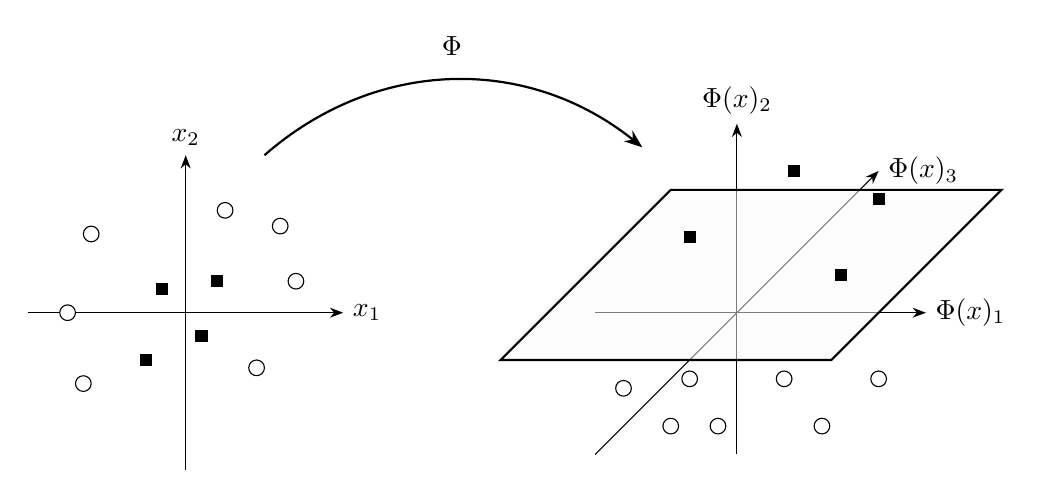
\begin{tikzpicture}[
        dot/.style={circle, draw=black, fill=white, inner sep=2pt},
        square/.style={rectangle, draw=black, fill=black, inner sep=2pt},
        >=Stealth
    ]
    % --- Left Side: Input Space (2D) ---
    \draw[->] (-2,0) -- (2,0) node[right] {$x_1$};
    \draw[->] (0,-2) -- (0,2) node[above] {$x_2$};
    % Circles
    \node[dot] at (-1.2, 1) {};
    \node[dot] at (0.5, 1.3) {};
    \node[dot] at (1.2, 1.1) {};
    \node[dot] at (1.4, 0.4) {};
    \node[dot] at (0.9, -0.7) {};
    \node[dot] at (-1.3, -0.9) {};
    \node[dot] at (-1.5, 0) {};
    % squares
    \node[square] at (-0.3, 0.3) {};
    \node[square] at (0.4, 0.4) {};
    \node[square] at (0.2, -0.3) {};
    \node[square] at (-0.5, -0.6) {};

    % --- The Mapping Arrow ---
    \draw[->, bend left=40, thick] (1, 2) to node[above=5pt] {$\Phi$} (5.8, 2.1);

    % --- Right Side: Feature Space (3D) ---
    \begin{scope}[xshift=7cm, yshift=0cm, scale=1.2]
        % 3D Axes
        \draw[->] (-1.5, 0) -- (2, 0) node[right] {$\Phi(x)_1$};
        \draw[->] (0, -1.5) -- (0, 2) node[above] {$\Phi(x)_2$};
        \draw[->] (-1.5, -1.5) -- (1.5, 1.5) node[right] {$\Phi(x)_3$};
        % Hyperplane
        \draw[thick, fill=gray!5, fill opacity=0.5] (-2.5, -0.5) -- (1, -0.5) -- (2.8, 1.3) -- (-0.7, 1.3) -- cycle;
        % Circles below the plane
        \node[dot] at (-1.2, -0.8) {};
        \node[dot] at (-0.2, -1.2) {};
        \node[dot] at (0.5, -0.7) {};
        \node[dot] at (0.9, -1.2) {};
        \node[dot] at (1.5, -0.7) {};
        \node[dot] at (-0.5, -0.7) {};
        \node[dot] at (-0.7, -1.2) {};
        % Squares above the plane
        \node[square] at (0.6, 1.5) {};
        \node[square] at (1.5, 1.2) {};
        \node[square] at (1.1, 0.4) {};
        \node[square] at (-0.5, 0.8) {};
    \end{scope}
    \end{tikzpicture}
    \caption{Mapping from 2D input space to 3D feature space using a polynomial feature map of degree 2.}
\end{figure}


\subsection{Linear separation in feature space}
Once the data is mapped into the feature space using the feature map $\phi$, we can apply SVM algorithms, replacing $\boldsymbol{x}$ with $\phi(\boldsymbol{x})$:
\begin{equation}
    f(x) = \boldsymbol{w}^T \phi(\boldsymbol{x}) + w_0
\end{equation}
A linear separation in the feature space corresponds to a non-linear separation in the original input space.
\\E.g. using the homogeneous polynomial feature map of degree $2$, the decision function becomes:
\[
    \phi\!\left(\begin{pmatrix} x_1 \\ x_2 \end{pmatrix}\right) = sgn(w_1 x_1^2 + w_2 x_1 x_2 + w_3 x_2^2 + w_0)
\]
The linear separator in the $3D$ feature space corresponds to a ellipse in the original $2D$ input space.
\begin{figure}[H]
    \centering
    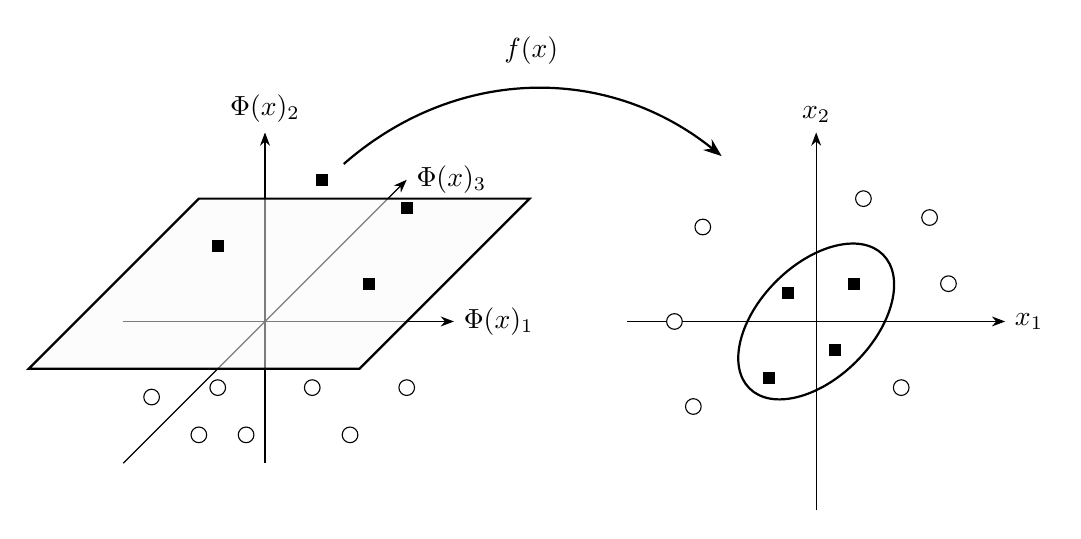
\begin{tikzpicture}[
        dot/.style={circle, draw=black, fill=white, inner sep=2pt},
        square/.style={rectangle, draw=black, fill=black, inner sep=2pt},
        >=Stealth
    ]
    \begin{scope}[xshift=0cm, yshift=0cm, scale=1.2]
        % 3D Axes
        \draw[->] (-1.5, 0) -- (2, 0) node[right] {$\Phi(x)_1$};
        \draw[->] (0, -1.5) -- (0, 2) node[above] {$\Phi(x)_2$};
        \draw[->] (-1.5, -1.5) -- (1.5, 1.5) node[right] {$\Phi(x)_3$};
        % Hyperplane
        \draw[thick, fill=gray!5, fill opacity=0.5] (-2.5, -0.5) -- (1, -0.5) -- (2.8, 1.3) -- (-0.7, 1.3) -- cycle;
        % Circles below the plane
        \node[dot] at (-1.2, -0.8) {};
        \node[dot] at (-0.2, -1.2) {};
        \node[dot] at (0.5, -0.7) {};
        \node[dot] at (0.9, -1.2) {};
        \node[dot] at (1.5, -0.7) {};
        \node[dot] at (-0.5, -0.7) {};
        \node[dot] at (-0.7, -1.2) {};
        % Squares above the plane
        \node[square] at (0.6, 1.5) {};
        \node[square] at (1.5, 1.2) {};
        \node[square] at (1.1, 0.4) {};
        \node[square] at (-0.5, 0.8) {};
    \end{scope}
        % --- The Mapping Arrow ---
        \draw[->, bend left=40, thick] (1, 2) to node[above=5pt] {$f(x)$} (5.8, 2.1);

        % --- Right Side: 2D space ---
        \begin{scope}[xshift=7cm, yshift=0cm, scale=1.2]
            \draw[->] (-2,0) -- (2,0) node[right] {$x_1$};
            \draw[->] (0,-2) -- (0,2) node[above] {$x_2$};
            % Circles
            \node[dot] at (-1.2, 1) {};
            \node[dot] at (0.5, 1.3) {};
            \node[dot] at (1.2, 1.1) {};
            \node[dot] at (1.4, 0.4) {};
            \node[dot] at (0.9, -0.7) {};
            \node[dot] at (-1.3, -0.9) {};
            \node[dot] at (-1.5, 0) {};
            % squares
            \node[square](d1) at (-0.3, 0.3) {};
            \node[square](d2) at (0.4, 0.4) {};
            \node[square](d3) at (0.2, -0.3) {};
            \node[square](d4) at (-0.5, -0.6) {};
            % Ellipse centered in 0,0 - x radius 1.5, y radius 1 - rotated 45 degrees counter-clockwise
            \draw[thick, black] (0,0) ellipse [x radius=1cm, y radius=0.6cm, rotate=45];
        \end{scope}
    \end{tikzpicture}
    \caption{Mapping from 2D input space to 3D feature space using a polynomial feature map of degree 2.}
    \label{fig:feature_map}
\end{figure}

\subsection{Kernel trick}
Computing the feature map $\phi(\boldsymbol{x})$ explicitly can be computationally expensive. 
However, this is not necessary to compute the SVM decision function.
\\In the \textbf{dual formulation} of SVMs (equations \ref{eq:svm_dual}, \ref{eq:soft_svm_dual}), the data points appear only in the form of \textbf{dot products} 
$\langle \phi(\boldsymbol{x}), \phi(\boldsymbol{x}') \rangle$.
\definition{Kernel trick}{
The \textbf{kernel trick} consists in replacing the dot product in the feature space with an equivalent \textbf{kernel function} 
    \begin{equation}
        \langle \phi ( \boldsymbol{x}), \phi (\boldsymbol{x}') \rangle
        = \phi(\boldsymbol{x})^T \phi(\boldsymbol{x}') 
        = k(\boldsymbol{x}, \boldsymbol{x}')
    \end{equation}
    The \textbf{kernel functions} uses examples in the \textbf{original input space} $\mathcal{X}$ 
    to compute the dot product in the \textbf{feature space} $\mathcal{H}$, 
    without explicitly computing the feature map $\phi$.
}
\subsubsection{Examples of kernels}
\paragraph{Homogeneous Polynomial Kernel}:
taking in consideration the equation \ref{eq:homogeneous_polynomial_feature_map}, we can derive the following kernel:
\begin{equation}
    k(\boldsymbol{x}, \boldsymbol{x}') = (\boldsymbol{x}^T \boldsymbol{x}')^d
\end{equation}
Setting $d=2$, we have:
\[
    k(\begin{pmatrix} x_1 \\ x_2 \end{pmatrix}, \begin{pmatrix} x_1' \\ x_2' \end{pmatrix}) = (x_1 x_1' + x_2 x_2')^2
\]
\[
    = (x_1 x_1')^2 + 2 x_1 x_2 x_1' x_2' + (x_2 x_2')^2
\]
\[
= \underbrace{(x_1^2, \sqrt{2} x_1 x_2, x_2^2)}_{\phi(\boldsymbol{x})^T}
\underbrace{
    \begin{pmatrix}
    x_1'^2 \\
    \sqrt{2} x_1' x_2' \\
    x_2'^2
    \end{pmatrix}
}_{\phi(\boldsymbol{x}')}
\]
This is equivalent to the dot product in the feature space defined by the homogeneous polynomial feature map of degree $2$, up to a scaling factor $\sqrt{2}$.

\paragraph{Non-Homogeneous Polynomial Kernel}:
\label{par:non_homogeneous_polynomial_kernel}
taking in consideration the equation \ref{eq:non_homogeneous_polynomial_feature_map}, we can derive the following kernel:
\begin{equation}
    k(\boldsymbol{x}, \boldsymbol{x}') = (\boldsymbol{x}^T \boldsymbol{x}' + 1)^d
\end{equation}
Setting $d=2$, we have:
\[
    k(\begin{pmatrix} x_1 \\ x_2 \end{pmatrix}, \begin{pmatrix} x_1' \\ x_2' \end{pmatrix}) = (x_1 x_1' + x_2 x_2' + 1)^2
\]
\[
    = (x_1 x_1')^2 + 2 x_1 x_1' x_2 x_2' + (x_2 x_2')^2 + 2 x_1 x_1' + 2 x_2 x_2' + 1
\]
\[ = \underbrace{(1, \sqrt{2} x_1, \sqrt{2} x_2, x_1^2, \sqrt{2} x_1 x_2, x_2^2)}_{\phi(\boldsymbol{x})^T}
\underbrace{
    \begin{pmatrix}
    1 \\
    \sqrt{2} x_1' \\
    \sqrt{2} x_2' \\
    x_1'^2 \\
    \sqrt{2} x_1' x_2' \\
    x_2'^2 \\
    \end{pmatrix}
}_{\phi(\boldsymbol{x}')}
\]
This is equivalent to the dot product in the feature space defined by the non-homogeneous polynomial feature map of degree $2$, up to a scaling factor $\sqrt{2}$.

\subsection{Valid Kernels}
\definition{Valid Kernel}{
    A kernel function $k : \mathcal{X} \times \mathcal{X} \to \mathbb{R}$ is valid if it corresponds to a dot product in some feature space $\mathcal{H}$:
    \begin{equation}
        k(\boldsymbol{x}, \boldsymbol{x}') = \langle \phi(\boldsymbol{x}), \phi(\boldsymbol{x}') \rangle
    \end{equation}
}
The kernel generalizes the concept of similarity between data points in arbitrary feature spaces.
\begin{figure}[H]
    \definition{Gram Matrix}{
        Given examples $\{\boldsymbol{x}_1, \boldsymbol{x}_2, \ldots, \boldsymbol{x}_m\}$, and a kernel function $k$, the \textbf{Gram matrix} $K$ is defined as:
        \begin{equation}
            K_{ij} = k(\boldsymbol{x}_i, \boldsymbol{x}_j) \forall i, j
        \end{equation}
        It can be interpreted as a matrix of pairwise similarities between the examples in the dataset,
        according to the kernel function $k$.
    }
\end{figure}

\definition{Positive definite matrix}{
    A symmetric matrix $K \in \mathbb{R}^{m \times m}$ is positive definite if:
    \begin{equation}
        \sum_{i,j = 1}^m c_i c_j K_{ij} \geq 0 \quad \forall \boldsymbol{c} \in \mathbb{R}^m
    \end{equation}
}
Equivalent definitions of positive definiteness include:
\begin{itemize}
    \item All eigenvalues of $K$ are non-negative;
    \item There exists a matrix $A$ such that $K = A^T A$.
\end{itemize}
A sufficient and necessary condition for a kernel $k$ to be valid is that 
the corresponding Gram matrix is positive definite for any choice of examples 
$\{\boldsymbol{x}_1, \boldsymbol{x}_2, \ldots, \boldsymbol{x}_m\}$.
There are several ways to check if a kernel is valid, e.g.:
\begin{itemize}
    \item Prove its positive definiteness;
    \item Find out a corresponding feature map $\phi$ (as we did before);
    \item Use kernel combination properties (e.g. sum, product yield valid kernels).
    This is the most common way to build complex kernels from simpler ones.
\end{itemize}
\subsubsection{Basic Kernels}
As just mentioned, basic kernels can be useful as building blocks for more complex kernels using kernel combination properties. 
Some common examples include:
\begin{itemize}
    \item \textbf{Linear Kernel}:
    \begin{equation}
        k(\boldsymbol{x}, \boldsymbol{x}') = \boldsymbol{x}^T \boldsymbol{x}'
    \end{equation}
    Apply no feature map, the kernel corresponds to the standard dot product in the input space.
    \item \textbf{Polynomial Kernel}:
    \begin{equation}
        k_{d,c}(\boldsymbol{x}, \boldsymbol{x}') = (\boldsymbol{x}^T \boldsymbol{x}' + c)^d
    \end{equation}
    The kernel depends on two parameters: the degree $d$ and the constant $c$. We have already seen this kernel
    in paragraph \ref{par:non_homogeneous_polynomial_kernel}.
    \item \textbf{Gaussian Kernel}:
    \begin{equation}
        k_\sigma(\boldsymbol{x}, \boldsymbol{x}') = \exp\left(-\frac{\|\boldsymbol{x} - \boldsymbol{x}'\|^2}{2\sigma^2}\right)
        = \exp\left(-\frac{\boldsymbol{x}^T \boldsymbol{x} + \boldsymbol{x}'^T \boldsymbol{x}' - 2 \boldsymbol{x}^T \boldsymbol{x}'}{2\sigma^2}\right) 
    \end{equation}
    The kernel depends on a parameter $\sigma$ that controls the width of the Gaussian function. The smaller the $\sigma$, the more localized the influence of each training example.
\end{itemize}
The Gaussian kernel is an example of \textbf{universal kernel}, which means that it can approximate any continuous function on a compact domain given enough data.
\subsubsection{Kernel Combinations}
Basic kernels can be \textbf{combined} using various operations to create more complex kernels from simpler ones. 
Correctly using combination operators guarantees that the resulting kernel is still positive definite.
\\We will now analyze some common kernel combination methods.
\subsubsection*{Kernel Sum}
The sum of two kernels corresponds to the concatenation of their feature spaces:
\begin{equation}
    k(\boldsymbol{x}, \boldsymbol{x}') = k_1(\boldsymbol{x}, \boldsymbol{x}') + k_2(\boldsymbol{x}, \boldsymbol{x}')
\end{equation}
Applying the definition of kernel:
\[
= \phi_1(\boldsymbol{x})^T \phi_1(\boldsymbol{x}') + \phi_2(\boldsymbol{x})^T \phi_2(\boldsymbol{x}')
\]
\[
= (\phi_1(\boldsymbol{x}) + \phi_2(\boldsymbol{x}))^T (\phi_1(\boldsymbol{x}') + \phi_2(\boldsymbol{x}'))
\]
\subsubsection*{Kernel Product}
The product of two kernels corresponds to the \textbf{cartesian product} of their features:
\begin{equation}
    (k_1 \times k_2)(\boldsymbol{x}, \boldsymbol{x}') = k_1(\boldsymbol{x}, \boldsymbol{x}') k_2(\boldsymbol{x}, \boldsymbol{x}')
\end{equation}
\[
= \sum_{i = 1}^n \phi_{1i}(\boldsymbol{x})\phi_{1i}(\boldsymbol{x}') \sum_{j = 1}^m \phi_{2j}(\boldsymbol{x})\phi_{2j}(\boldsymbol{x}')
\]
\[
= \sum_{i = 1}^n \sum_{j = 1}^m (\phi_{1i}(\boldsymbol{x}) \phi_{2j}(\boldsymbol{x})) (\phi_{1i}(\boldsymbol{x}') \phi_{2j}(\boldsymbol{x}'))
\]
\[
= \sum_{k = 1}^{nm} \phi_{12k}(\boldsymbol{x}) \phi_{12k}(\boldsymbol{x}') = \phi_{12}(\boldsymbol{x})^T \phi_{12}(\boldsymbol{x}')
\]
where $\phi_{12}(\boldsymbol{x}) = \phi_{1}(\boldsymbol{x}) \times \phi_{2}(\boldsymbol{x})$ is the cartesian product of the two feature maps.
The product can also be between kernel in different spaces.
\subsubsection*{Linear combination of kernels}
A kernel can be rescaled by a positive constant:
\[ k_{\beta}(\boldsymbol{x}, \boldsymbol{x}') = \beta k(\boldsymbol{x}, \boldsymbol{x}')\]
We can define a linear combination of kernels as:
\[k_{sum}(\boldsymbol{x}, \boldsymbol{x}') = \sum_{k=1}^K \beta_k k_k(\boldsymbol{x}, \boldsymbol{x}') \]
Since understanding what kernel works best for a given problem can be challenging, combining multiple kernels allows us to leverage the strengths of each individual kernel.
With \textbf{kernel learning} the weights $\beta_k$ of the combination can be learned from data, allowing the model to adaptively combine multiple kernels.
\subsubsection*{Kernel Normalization}
Kernel values can be influenced by the dimension of objects. I.E., in text classification, longer documents tend to have higher dot products simply because they contain more words.
\\To mitigate this effect, we can normalize the kernel:
\begin{equation}
    \hat{k}(\boldsymbol{x}, \boldsymbol{x}') = \frac{k(\boldsymbol{x}, \boldsymbol{x}')}{\sqrt{k(\boldsymbol{x}, \boldsymbol{x}) k(\boldsymbol{x}', \boldsymbol{x}')}}
\end{equation}
This is a \textbf{cosine normalization}, which takes into account the angle between the feature vectors rather than their magnitudes.
\subsection{Kernel on Graphs}
Kernels on graphs heavily rely on the Weisfeiler-Lehman (WL) test for graph isomorphism.
\subsubsection{Graph Isomorphism}
To understand this algorithm, we need to define the concept of \textbf{graph isomorphism}.
\definition{Graph Isomorphism}{
    Two graphs $G = (V, E)$ and $G' = (V', E')$ are isomorphic if there exists a bijection $f: V \to V'$ such that:
    \begin{equation}
        (u, v) \in E \iff (f(u), f(v)) \in E'
    \end{equation}
}
In a nutshell, two graphs are isomorphic if they have the same structure, but possibly different node labels.
\subsubsection{Weisfeiler-Lehman Test}
If isomorphism is easy to check on vectorial data, it is much more challenging on graph data. This is in fact an NP-hard problem.
\\The WL test is an approximate algorithm that can efficiently determine if two graphs are non-isomorphic, but it may fail to distinguish some non-isomorphic graphs (false positives).
\paragraph{Algorithm:}
We are now going to present the WL algorithm on two graphs with same node labels:
\begin{itemize}
    \item Given two graphs $G = (V, E)$ and $G' = (V', E')$ with $|V| = |V'| = n$;
    \item Let $L(G) = {l(v)| v \in V} $ be the set of node labels in $G$. $l(v)$ is a function returning the label of node $v$; 
    \item Let $L(G') = L(G)$;
    \item Let $label(s)$ be a function assigning a unique label to a string.
\end{itemize}
The algorithm is defined as follows:
\begin{algorithm}[H]
    \caption{Weisfeiler-Lehman Test}
    \begin{algorithmic}
        \State Set $l_0(v) \leftarrow l(v), \forall v \in V$
        \For{$i = 1$ to $n-1$}
            \For{each node $v \in G$}
                \State Let $M_i(v) = \{l_{i-1}(u) | u \in \text{neigh}(v)\}$
                \State Concatenate the sorted labels of $M_i(v)$ into $s_i(v)$
                \State Let $l_i(v) = label(l_{i-1}(v) \oplus s_i(v))$
            \EndFor
            \State If $L_i(G) \neq L_i(G')$, return \textbf{not isomorphic}
        \EndFor
        \State Return \textbf{possibly isomorphic}
    \end{algorithmic}
\end{algorithm}
Where:
\begin{itemize}
    \item $M_i(v)$: the multiset of labels of the neighbors of node $v$ at iteration $i$;
    \item $l_i(v)$: the new label assigned to node $v$ at iteration $i$. It is computed by assigning a unique label 
    to the concatenation of the previous label $l_{i-1}(v)$ and the sorted labels of its neighbors $s_i(v)$.
\end{itemize}
\subsubsection{Weisfeiler-Lehman Kernel}
\begin{itemize}
    \item Let ${G_1, G_2, \ldots, G_h} = {(V, E, l_0), (V, E, l_1), \ldots, (V, E, l_h)}$ be a set of resulting graphs after applying $h$ iterations of the WL algorithm on graph $G$.
    \item Let $k: G \times G \to \mathbb{R}$ be any kernel on graphs;
\end{itemize}
The \textbf{Weisfeiler-Lehman kernel} between two graphs $G$ and $G'$ is defined as:
\begin{equation}
    K_{WL}^{h}(G, G') = \sum_{i=0}^h k(G_i, G_i')
\end{equation}

\include{sections/NeuralNetworks.tex}
\include{sections/Clustering.tex}
\include{sections/ReinforcementLearning.tex}
\include{sections/Ensemble-methods.tex}
\appendix
\section{Principal Component Analysis}
\label{sec:PCA}
Principal Component Analysis (PCA) is a widely used technique for dimensionality reduction and 
feature extraction in machine learning and statistics.
Let $\boldsymbol{X} \in \mathbb{R}^{n \times d}$ be a data matrix, with correlated coordinates.
PCA is a linear transformation that transforms the data into a new coordinate system of uncorrelated variables.
\subsection{PCA Algorithm}
The PCA algorithm can be summarized in the following steps:
\begin{enumerate}
    \item Compute the \textbf{mean} of the data:
    \begin{equation}
        \bar{\boldsymbol{x}} = \frac{1}{n} \sum_{i = 1}^{n} \boldsymbol{x}_i
    \end{equation}
    \item Center the data by subtracting the mean from each data point:
    \begin{equation}
        \boldsymbol{X} = \boldsymbol{X} - \bar{\boldsymbol{x}}
    \end{equation}
    We are basically defining a new matrix, where each row is the original data point minus the mean.
    \item Compute the \textbf{covariance matrix} of the centered data:
    \begin{equation}
        \boldsymbol{C} = \frac{1}{n} \boldsymbol{X}^T \boldsymbol{X}
    \end{equation}
    Since $x_i = x_i - \bar{x}$, this is equivalent to the usual definition of covariance.
    In fact, we have:
    \[
     X^T X = \sum_{i=1}^{n} \boldsymbol{x}_i \boldsymbol{x}_i^T = \sum_{i=1}^{n} (\boldsymbol{x}_i - \bar{\boldsymbol{x}})(\boldsymbol{x}_i - \bar{\boldsymbol{x}})^T = \sum_{i = 1}^{n} (\boldsymbol{x}_i - \bar{\boldsymbol{x}})^2
    \]
    \item Compute the \textbf{eigenvalues} and \textbf{eigenvectors} of the covariance matrix $\boldsymbol{C}$.
    The eigenvectors represent the directions of maximum variance in the data, 
    while the eigenvalues indicate the amount of variance in the direction of each eigenvector.
    \item We can then select the top $k$ eigenvectors corresponding to the largest eigenvalues
    to form a new feature space of reduced dimensionality.
\end{enumerate}

\end{document}
